% !TEX root = ./main.tex
% !TEX encoding = UTF-8 Unicode
% !TEX program = pdflatex
% !TeX spellcheck = it_IT

\chapter{Analisi dei risultati}
In questo capitolo saranno mostrati i risultati ottenuti per ogni combinazione
lineare utilizzata.

\section{Scelta dei parametri di Scoring}
Per il tuning dei parametri di scoring si è eseguito l'intero processo più volte
mirando ad ottenere la combinazione che presentasse la copertura del grafo
maggiore.\\
In \figurename~\ref{} è riportata la tabella contenente i test effettuati.

\begin{figure}[!htbp]
  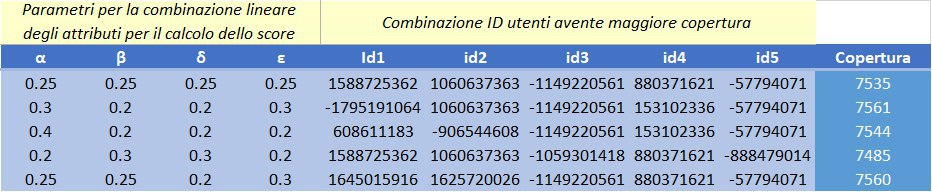
\includegraphics[width=1\linewidth,keepaspectratio]{ris_table}
  \caption{Tabella Risultati}
  \label{ris_table}
\end{figure}
